\chapter{User Guide}
\label{ch:appendix_user_guide}
In this short user guide, we show how to use our proof-of-concept implementation step by step.

\section{Signing a Document}\label{sec:signing-a-document}
This section contains a step by step guide on how to obtain a signature for a document.

\subsection{Ready the Document}\label{subsec:ready-the-document}
The first step is to make sure the document is ready.

We \textbf{strongly} recommend using a read-only format,
such as \gls{PDF},
as the slightest change to the source document will invalidate its signature.
Some editors even modify the document if it is simply opened for viewing,
such as Microsoft Word.

If the document is ready for signing, navigate to the signing server using the preferred web browser.
Whether a desktop, a laptop, a mobile device such as a smartphone or a tablet is used doesn't matter.

The frontend will present itself as shown in figure~\ref{fig:userguide0}.
\begin{figure}[H]
    \begin{center}
        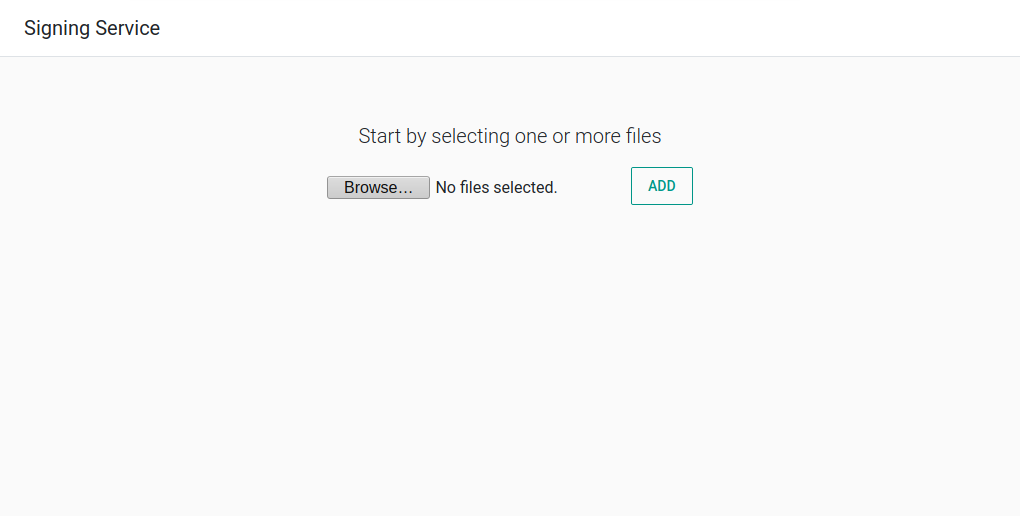
\includegraphics[width=\linewidth]{images/userguide_sign_0.png}
    \end{center}
    \caption{The frontend of the signing server upon initial access}
    \label{fig:userguide0}
\end{figure}

\subsection{Submit the Document for Hashing}\label{subsec:submit-the-document-for-hashing}
The next step is to submit the document for hashing.
Click the button labelled "Browse" and select the document to be signed.

The signing of multiple documents at once is supported as well.
If multiple documents are to be signed together,
simply select them all.

The frontend will look like as shown in figure~\ref{fig:userguide1}.

\begin{figure}[H]
    \begin{center}
        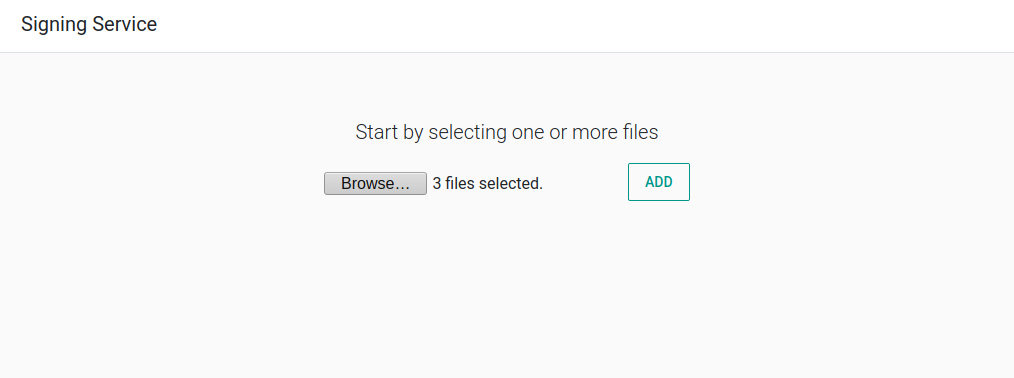
\includegraphics[width=\linewidth]{images/userguide_sign_1.png}
    \end{center}
    \caption{The frontend of the signing server after selecting the documents to sign}
    \label{fig:userguide1}
\end{figure}

Then click the green button labelled "Add".
The frontend will immediately begin hashing them.
It will show the progress for each file as it is processing it,
then display the hash value,
for double-checking by the user,
if so desired.

Please note that no data whatsoever leaves the device at this point.
All operations are performed purely in-browser.

Figure~\ref{fig:userguide2} illustrates what the frontend looks like during document hashing.

\begin{figure}[H]
    \begin{center}
        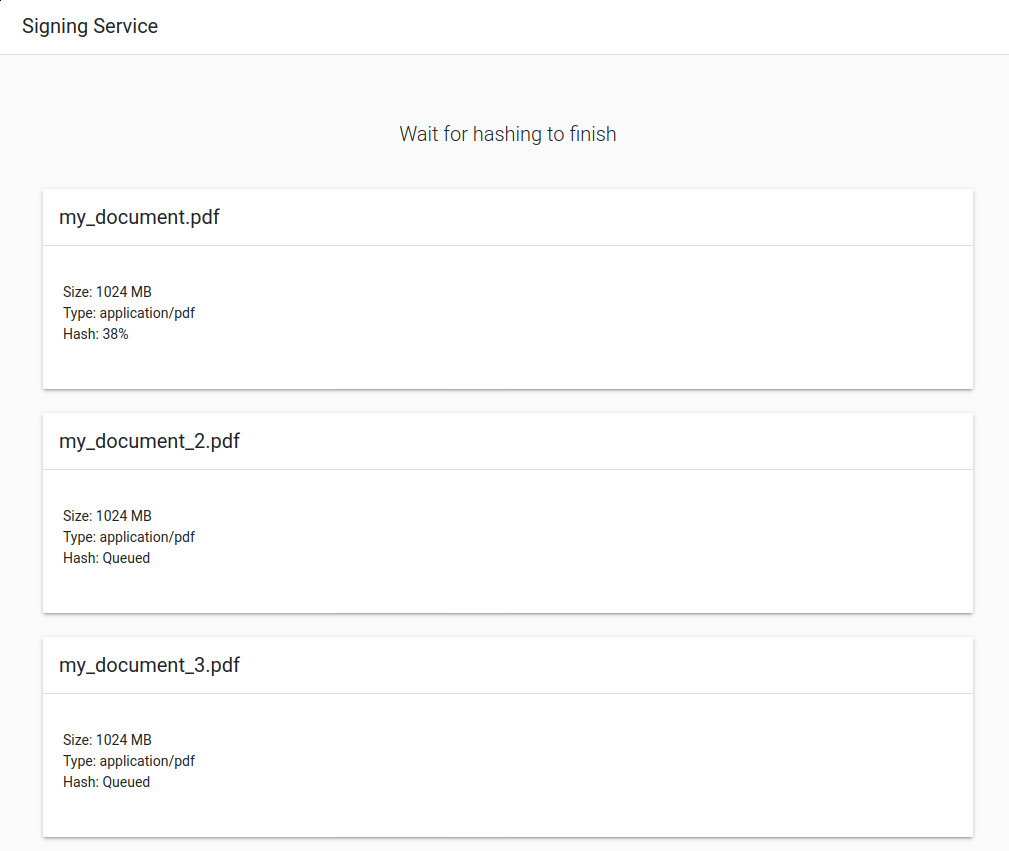
\includegraphics[width=\linewidth]{images/userguide_sign_2.png}
    \end{center}
    \caption{The frontend of the signing server when hashing}
    \label{fig:userguide2}
\end{figure}

When hashing is completed, the frontend will offer to submit the hashes to the signing server.
Figure~\ref{fig:userguide3} illustrates what this looks like.

\begin{figure}[H]
    \begin{center}
        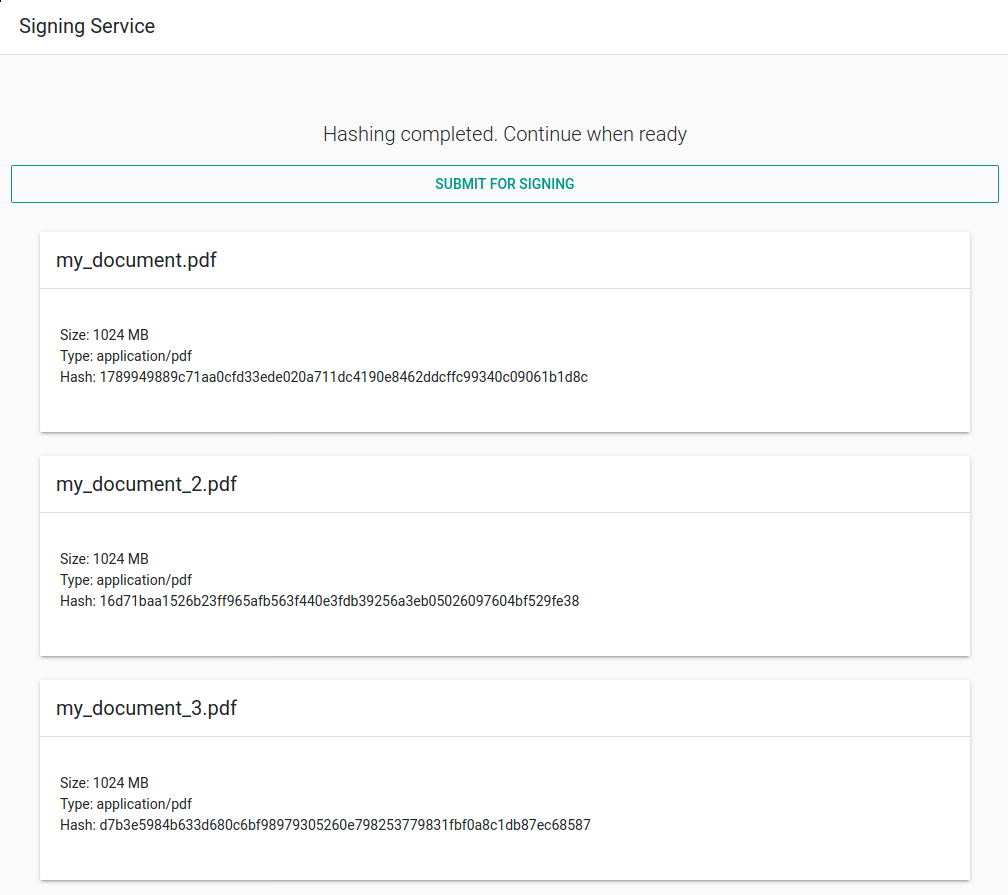
\includegraphics[width=\linewidth]{images/userguide_sign_3.png}
    \end{center}
    \caption{The frontend of the signing server upon completion of hashing}
    \label{fig:userguide3}
\end{figure}

When ready, press the green button labelled "Submit for Signing".
The hashes will be submitted to the signing server.

\subsection{Selecting an IDP and Authenticating}\label{subsec:selecting-an-idp-and-authenticating}
The signing server will respond with a list of the \gls{IDP} it trusts,
which are displayed as buttons, as shown in figure~\ref{fig:userguide4}.


\begin{figure}[H]
    \begin{center}
        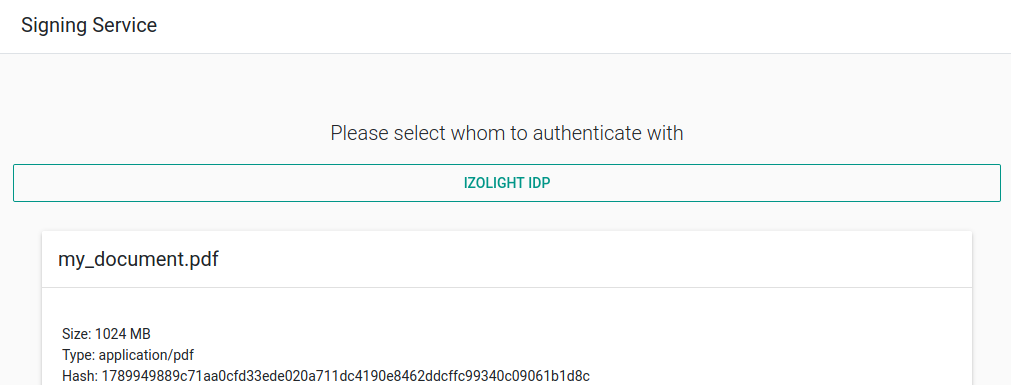
\includegraphics[width=\linewidth]{images/userguide_sign_4.png}
    \end{center}
    \caption{The frontend of the signing server offering the choices of IDPs}
    \label{fig:userguide4}
\end{figure}

If there's only one \gls{IDP}, only one button is displayed.
Click on the button representing the preferred \gls{IDP}.
This will start the authentication process.

What the next steps look like depends on the \gls{IDP}.
In our demo \gls{IDP}, the login screen looks like shown in figure~\ref{fig:userguide5}.

\begin{figure}[H]
    \begin{center}
        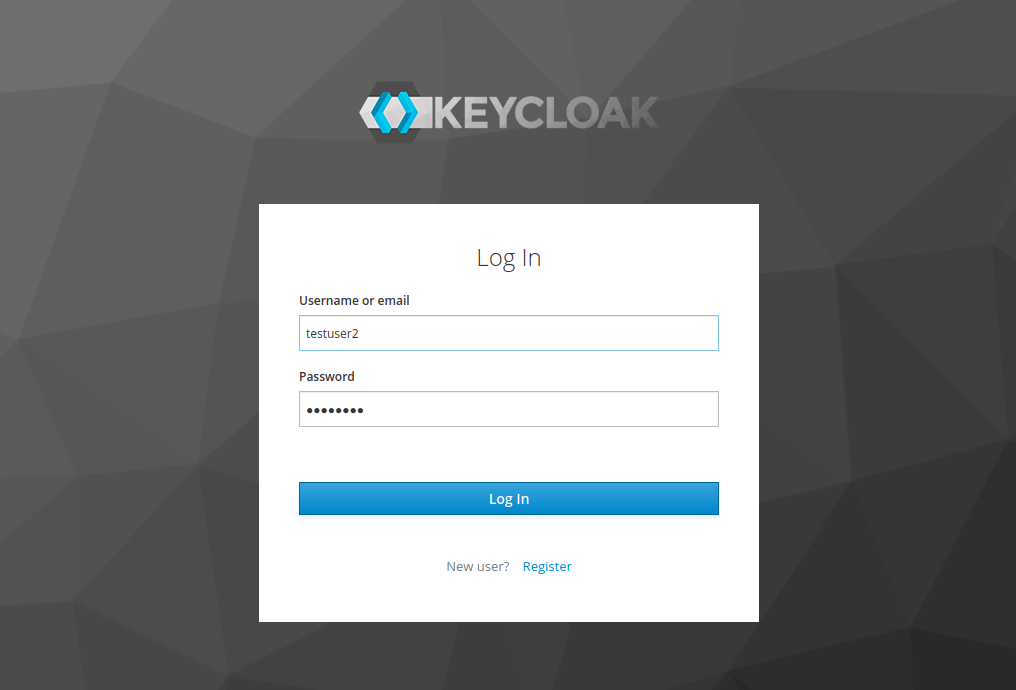
\includegraphics[width=\linewidth]{images/userguide_sign_5.png}
    \end{center}
    \caption{The IDP asking for credentials}
    \label{fig:userguide5}
\end{figure}

Provide the credentials and multi-factor tokens as required by the \gls{IDP}.
Upon successful authentication,
the signing server will begin creating the signature.

\subsection{Retrieving the Created Signature}\label{subsec:retrieving-the-created-signature}
This may take a few seconds, depending on server load.

During signature creation, the frontend looks like shown in figure~\ref{fig:userguide6}.

\begin{figure}[H]
    \begin{center}
        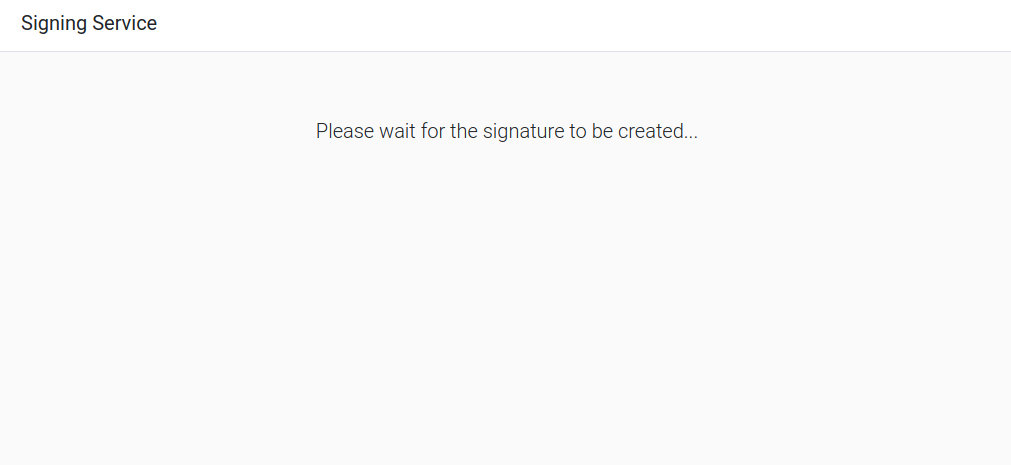
\includegraphics[width=\linewidth]{images/userguide_sign_6.png}
    \end{center}
    \caption{Signature creation in progress}
    \label{fig:userguide6}
\end{figure}

When signature creation is completed,
a file download button will appear.
Click the button,
and a file download will be launched,
as shown in figure~\ref{fig:userguide6}.


\begin{figure}[H]
    \begin{center}
        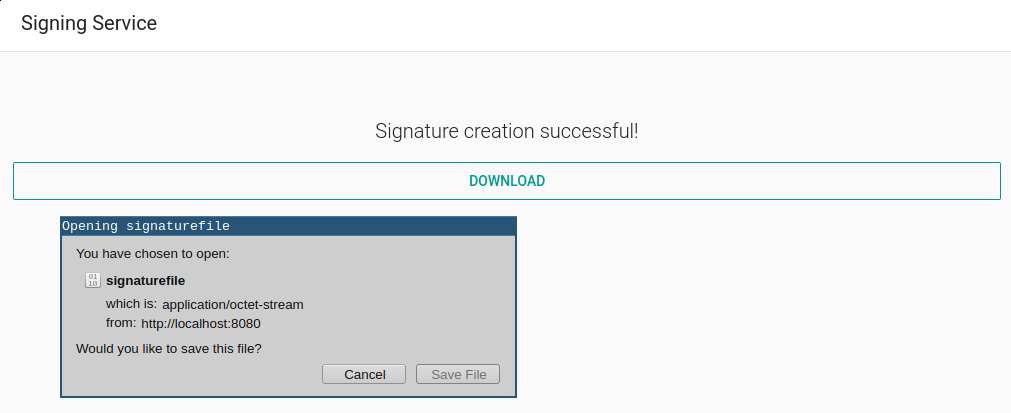
\includegraphics[width=\linewidth]{images/userguide_sign_7.png}
    \end{center}
    \caption{Signature file download}
    \label{fig:userguide7}
\end{figure}

Make sure to save the signature file,
for it is not persisted on the server indefinitely.

Congratulations!
The signature has been created successfully.





\section{Verifying a Signature}\label{sec:verifying-a-signature}
This section contains a step by step guide on how to verify a signature that was previously created.

\subsection{Ready the Document and Its Signature File}\label{subsec:ready-the-document-and-its-signature-file}
The first step is to make the document and its signature file is at hand.

If the document is ready for verification, navigate to the verification service using the preferred web browser.
The verification service may be running either in an internet-accessible location,
or on the local machine.
For devices such as tablets and smartphones running Android or iOS,
only online verification is supported.
For devices such as laptops and desktops running GNU/Linux, Mac OS X or Windows,
offline verification is supported by launching the appropriate build of the verifier program on the local machine.

Whether the verification service is accessed locally or not doesn't matter for the steps that follow,
the procedure remains the same.

Upon accessing the verification service, its frontend will present itself as shown in figure~\ref{fig:verify0}.
\begin{figure}[H]
    \begin{center}
        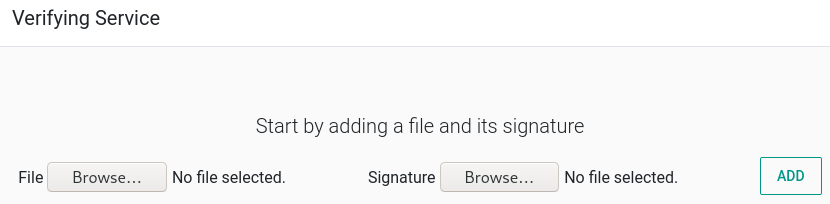
\includegraphics[width=\linewidth]{images/userguide_verify_0.png}
    \end{center}
    \caption{The frontend of the verification service upon initial access}
    \label{fig:verify0}
\end{figure}

Proceed by selecting first the document, and then its signature to begin the verification process.


After selecting the files, press the green "Add" button.
The frontend will start hashing the document.
When hashing is completed,
the document's hash and the signature file are ready for transmission to the verification service,
as shown in figure~\ref{fig:verify1}.


Please note that no matter how the verification service is used,
remote or local,
mobile device or not,
the document never leaves the device.

\begin{figure}[H]
    \begin{center}
        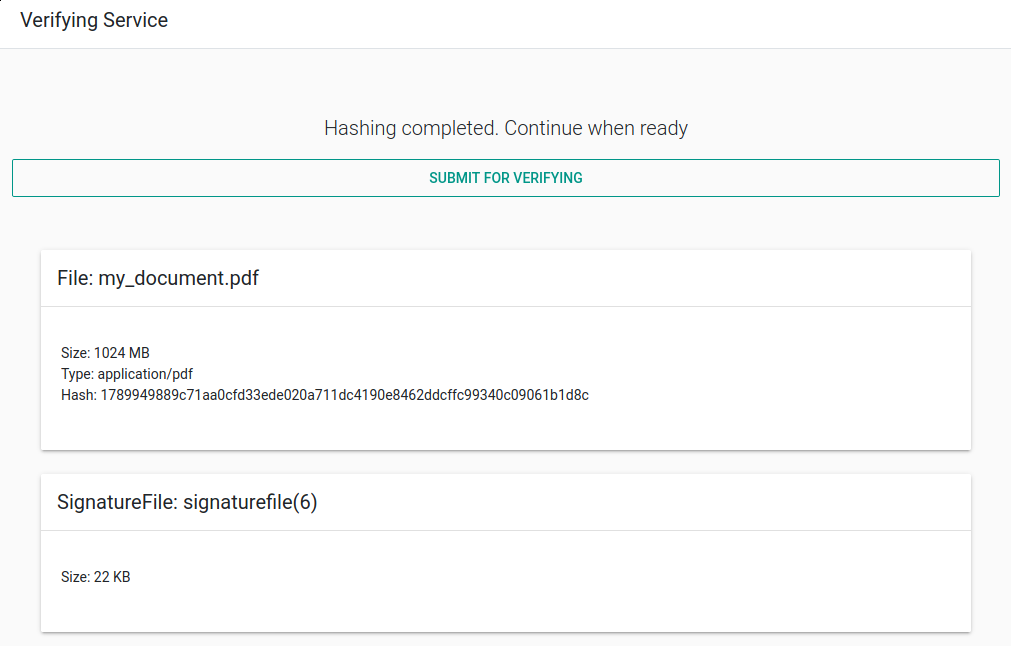
\includegraphics[width=\linewidth]{images/userguide_verify_1.png}
    \end{center}
    \caption{Verification service ready for verification}
    \label{fig:verify1}
\end{figure}

\subsection{Submit Document and Signature File for Verification}\label{subsec:submit-document-and-signature-file-for-verification}

When ready for submission, press the green button labelled "submit for verifying".

The verification service will then attempt to verify the signature.
If signature verification was successful,
the verification service will display a result as shown in figure~\ref{fig:verify2}.


\begin{figure}[H]
    \begin{center}
        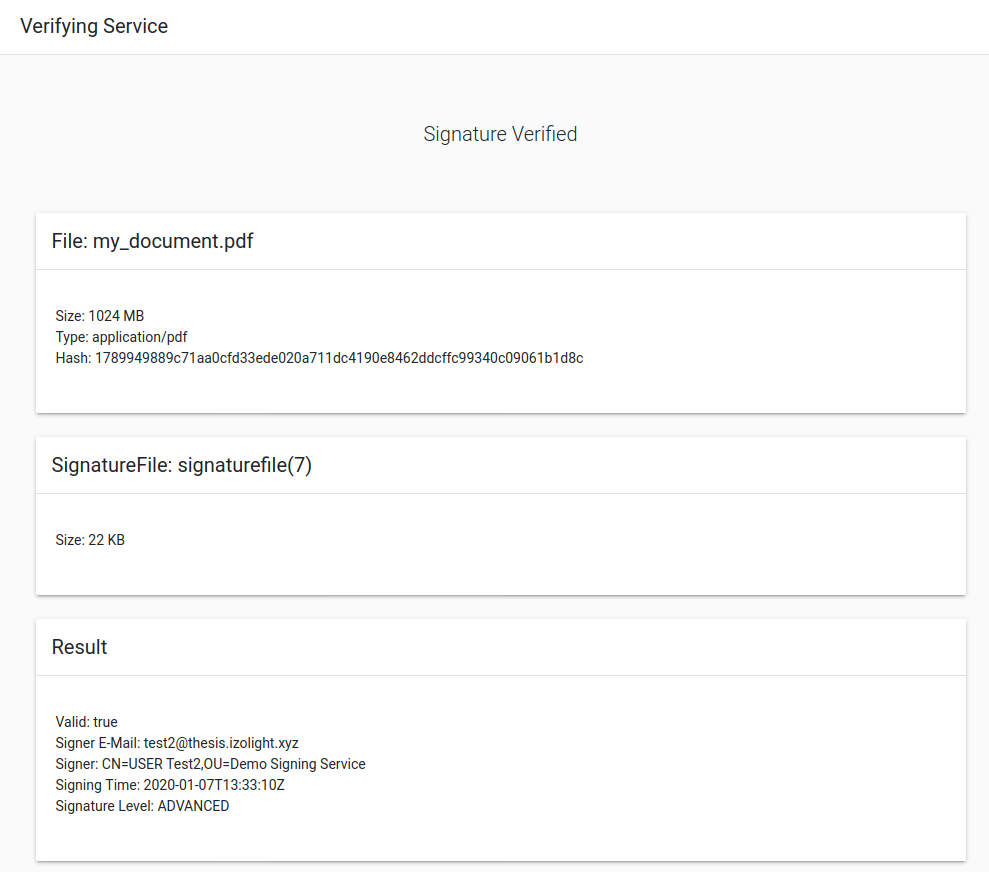
\includegraphics[width=\linewidth]{images/userguide_verify_2.png}
    \end{center}
    \caption{Verification service has completed verification}
    \label{fig:verify2}
\end{figure}

For verification of another document as part of the same signature,
the procedure is exactly the same,
simply select the other document together with the same signature file as above.

Congratulations!
The signature has been verified successfully.
